\documentclass[runningheads]{llncs}

\usepackage{graphicx}
\usepackage{amsmath}
\usepackage{booktabs}
\usepackage{hyperref}

\begin{document}

\title{Real-Time Human Behavior Analysis for Theft and Vandalism Detection Using YOLOv11 and Deep Learning}

\author{
Debashish Kashyap\inst{1} \and
Nilkamal Borah\inst{1} \and
Anjan Kumar Talukdar\inst{1}
}

\authorrunning{D. Kashyap et al.}

\institute{
Gauhati University, Guwahati-781014, Assam, India
}

\maketitle

\begin{abstract}
This paper presents a real-time surveillance system for detecting theft, vandalism, fighting, and normal behavior using a hybrid deep learning pipeline. The system integrates YOLOv11 for frame-level object detection and an InceptionV3+GRU network for temporal video-level classification. A custom multi-class dataset was collected and annotated with bounding boxes. The YOLOv11 component achieves mAP@50 of 0.96, precision of 0.95, and recall of 0.93. An automated Telegram alert module enables immediate incident notification. The system operates in real time on a consumer-grade GPU, demonstrating its suitability for scalable deployment in smart public surveillance environments.

\keywords{YOLOv11 \and Human Behavior Analysis \and Theft Detection \and Vandalism Detection \and CNN+LSTM \and Computer Vision \and Real-Time Surveillance}
\end{abstract}

\section{Introduction}

The proliferation of closed-circuit television (CCTV) cameras in public and private spaces has created an enormous volume of surveillance footage that exceeds the capacity of manual monitoring. Traditional surveillance systems rely heavily on human operators, who are susceptible to fatigue, distraction, and oversight, leading to delayed or missed responses to criminal incidents. Automated intelligent surveillance systems that leverage computer vision and deep learning offer a scalable alternative capable of continuous, consistent monitoring.

Recent advances in deep learning, particularly convolutional neural networks (CNNs) and recurrent neural networks (RNNs), have significantly improved the accuracy and speed of activity recognition and object detection systems~\cite{he2016,simonyan2015}. Object detection frameworks such as the YOLO (You Only Look Once) family~\cite{redmon2016,jocher2023} have enabled real-time detection on commodity hardware by formulating detection as a single regression problem rather than a multi-stage pipeline. The most recent variant, YOLOv11~\cite{khanam2024}, introduces further improvements in architecture efficiency and detection accuracy.

Despite these advances, detecting fine-grained behaviors such as theft and vandalism remains challenging due to intra-class variation, occlusion, and the need to capture temporal dynamics across frames. A purely frame-level detector may miss activities that manifest only over a sequence of frames, motivating the use of video-level sequence models.

This paper proposes a hybrid real-time behavior analysis system that addresses these challenges by combining:
\begin{itemize}
    \item \textbf{YOLOv11} for frame-level detection and bounding-box localization of suspicious activities.
    \item \textbf{InceptionV3 + GRU (CNN+LSTM)} for video-level temporal classification across the four behavior categories.
    \item \textbf{Automated Telegram alerts} for immediate real-time notification upon detection of a suspicious event.
\end{itemize}

The remainder of the paper is organized as follows. Section~\ref{sec:related} reviews related work. Section~\ref{sec:method} describes the proposed methodology. Section~\ref{sec:results} presents experimental results, and Section~\ref{sec:conclusion} concludes the paper.

\section{Related Work}
\label{sec:related}

Object detection for anomaly and crime detection has been an active research area. Redmon et al.~\cite{redmon2016} introduced the YOLO architecture, enabling real-time single-pass detection. Successive versions (YOLOv3–YOLOv8) continued to improve both speed and accuracy. YOLOv11~\cite{khanam2024} refines the backbone and neck design, achieving higher accuracy with fewer parameters.

For temporal activity recognition, CNN+RNN hybrid architectures have demonstrated strong performance. Donahue et al.~\cite{donahue2015} showed that combining CNNs for spatial feature extraction with LSTMs for temporal modeling yields competitive results on action recognition benchmarks. Simonyan and Zisserman~\cite{simonyan2015} introduced two-stream networks exploiting both appearance and optical flow. More recently, 3D convolution (C3D) and transformer-based methods have been explored, though they impose higher computational costs.

For theft and shoplifting detection specifically, prior work has exploited skeleton-based pose estimation, optical flow, and CNN-based frame classifiers. However, few systems combine a real-time frame-level detector with a video-level classifier and an automated alert mechanism, as proposed here.

\section{Proposed Methodology}
\label{sec:method}

The overall pipeline of the system is illustrated in Fig.~\ref{fig:block}. The input video stream is processed by two parallel modules: a YOLOv11-based frame detector and an InceptionV3+GRU video classifier. Upon detection of a suspicious activity, the alert module sends a notification via a Telegram bot.

\begin{figure}[t]
\centering
\fbox{\parbox{0.9\textwidth}{\centering\vspace{1cm}
\textbf{Video Input} $\longrightarrow$ \textbf{Frame Extraction} $\longrightarrow$ \textbf{YOLOv11 Detector}\\[6pt]
\hspace{6cm}$\searrow$\\[4pt]
\hspace{6cm}\textbf{InceptionV3 + GRU Classifier}\\[6pt]
\hspace{6cm}$\downarrow$\\[4pt]
\hspace{6cm}\textbf{Telegram Alert System}
\vspace{1cm}}}
\caption{Block diagram of the hybrid theft and vandalism detection system.}
\label{fig:block}
\end{figure}

\subsection{Dataset and Annotation}

The dataset was assembled from publicly available video sources and custom recordings. It contains four activity classes: \textit{normal}, \textit{theft}, \textit{vandalism}, and \textit{fighting}. For the YOLO training pipeline, individual frames were extracted and annotated with axis-aligned bounding boxes using the YOLO label format. Each annotation specifies the class index and normalized box coordinates $(c_x, c_y, w, h)$.

Figure~\ref{fig:labels} shows the class and bounding-box distribution of the training set. The dataset is split into training, validation, and test subsets following an approximately 70/15/15 ratio.

\begin{figure}[t]
\centering
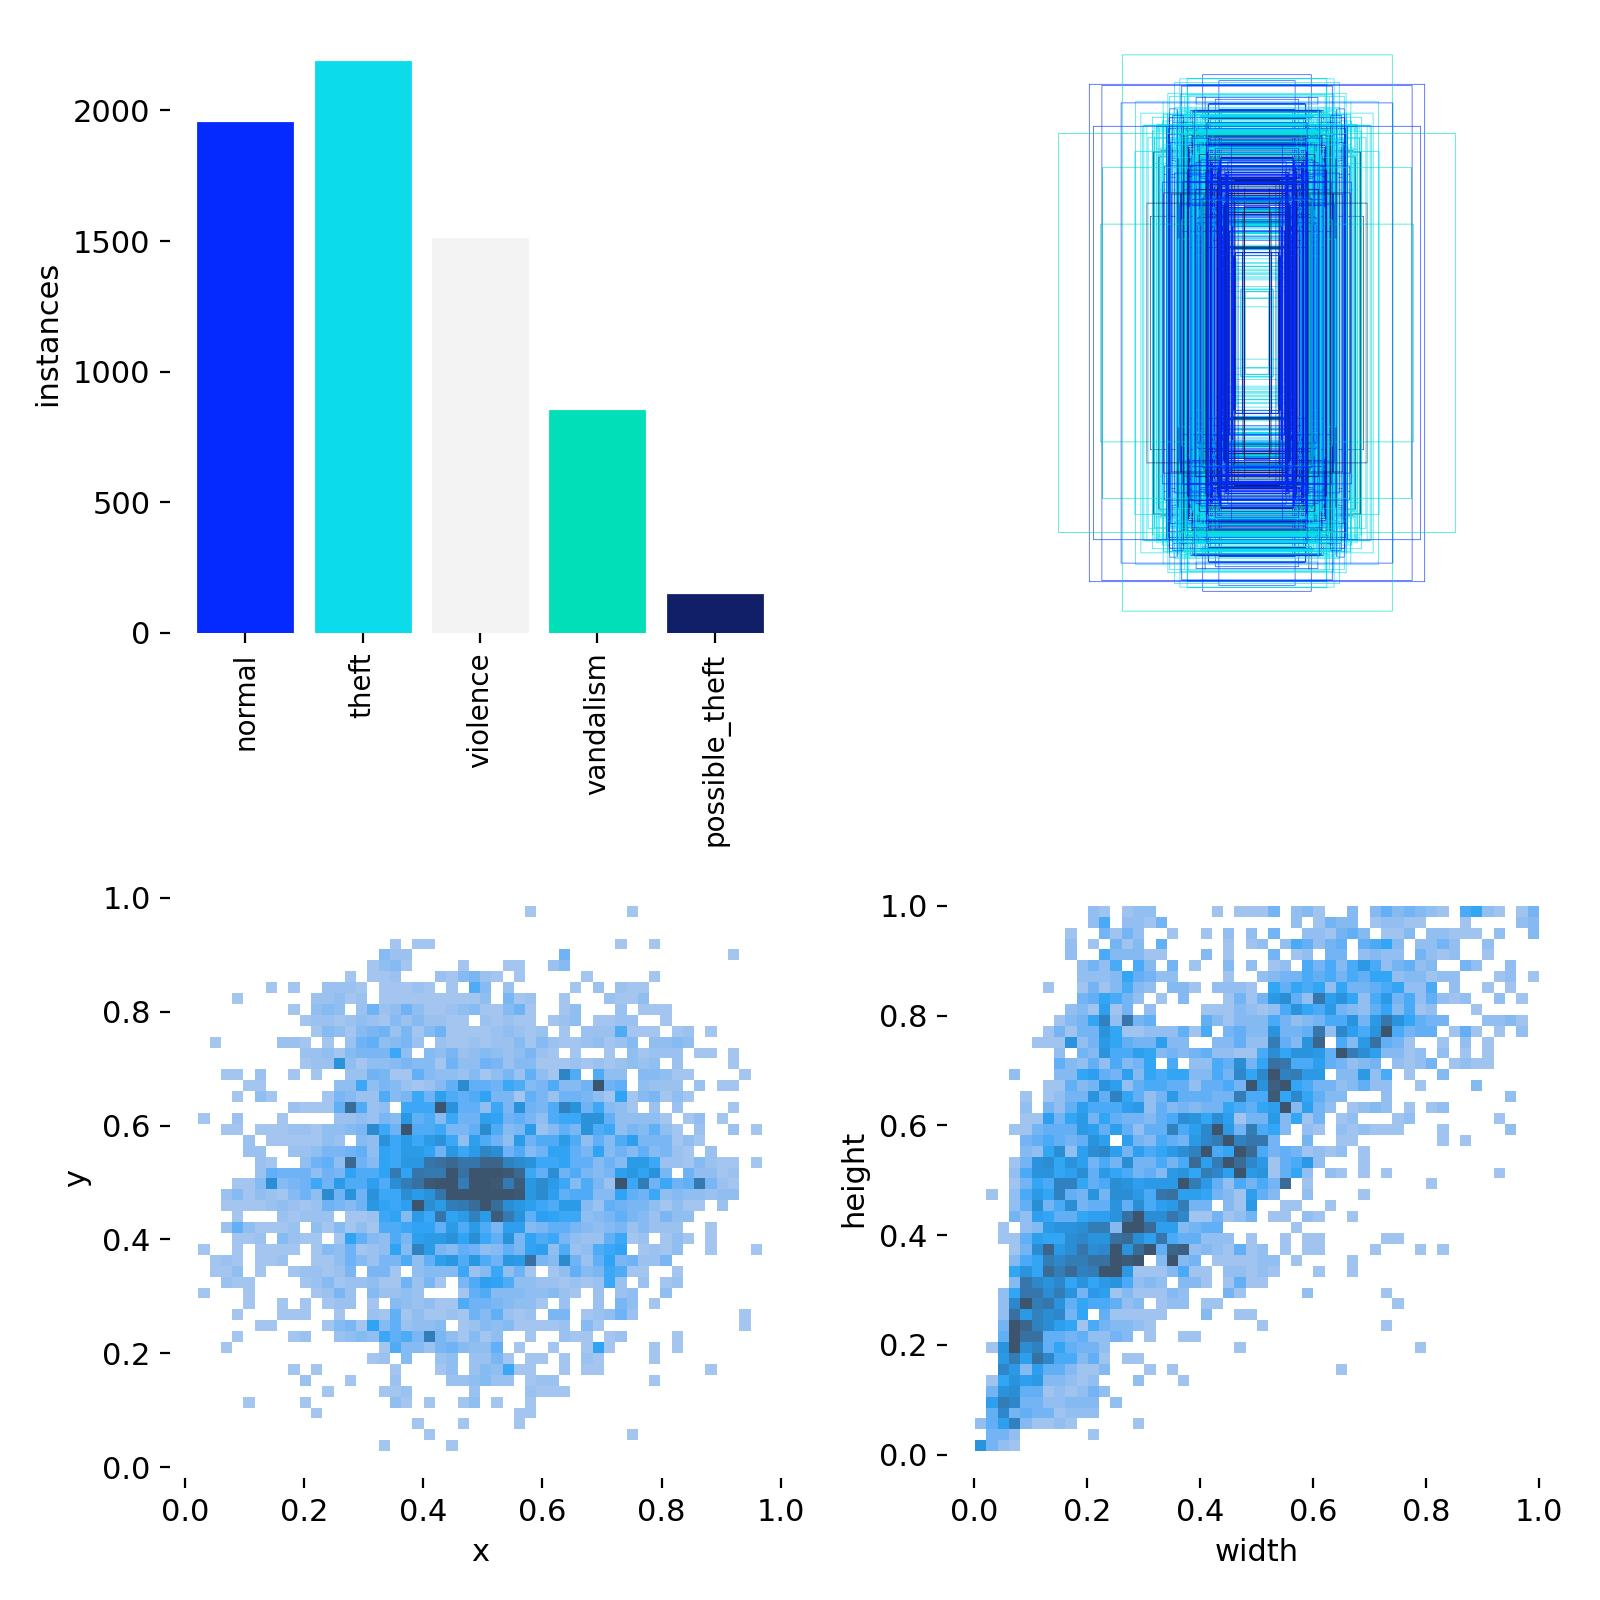
\includegraphics[width=0.85\textwidth]{labels.jpg}
\caption{Dataset label distribution and bounding-box statistics across the four behavior classes.}
\label{fig:labels}
\end{figure}

For the CNN+LSTM pipeline, full video clips are used. Training employs 34 video sequences and testing employs 13 sequences across three classes: normal, theft, and fighting. Vandalism clips were incorporated into the YOLO detection branch; expanding the video classifier to all four classes is reserved for future work as additional labeled video data are collected.

\subsection{Data Augmentation}

To reduce overfitting and improve generalization, the following augmentation techniques were applied during YOLO training:
\begin{itemize}
    \item Horizontal flip and random rotation ($\pm15^\circ$).
    \item Brightness and contrast jitter.
    \item Mosaic augmentation (four-image composition) at the batch level.
    \item Random scale and crop within the input resolution of $640 \times 640$.
\end{itemize}
For the video classification branch, temporal sub-sampling was used to extract up to 20 evenly spaced frames per clip, providing robustness to varying clip lengths.

\subsection{YOLOv11 Object Detection Module}

YOLOv11 (YOLOv11n variant) was selected as the detection backbone due to its favorable trade-off between inference speed and accuracy. The model was initialized from pretrained ImageNet weights and fine-tuned on the custom surveillance dataset. Training configuration:

\begin{itemize}
    \item \textbf{Epochs}: 200
    \item \textbf{Batch size}: 12
    \item \textbf{Image size}: $640 \times 640$
    \item \textbf{Hardware}: NVIDIA GeForce GTX 1650 (CUDA 12.7)
    \item \textbf{Optimizer}: SGD with cosine learning-rate schedule
\end{itemize}

The model outputs bounding boxes, class probabilities, and confidence scores per detected object. Detections with a confidence below 0.3 are suppressed using non-maximum suppression (NMS).

\subsection{CNN+LSTM Video Classification Module}

For video-level classification, a two-stage pipeline is employed:

\begin{enumerate}
    \item \textbf{Feature extraction}: Each frame is passed through InceptionV3 (pretrained on ImageNet, global average pooling head) to produce a 2048-dimensional feature vector.
    \item \textbf{Sequence modeling}: The per-frame feature sequences (up to $T = 20$ frames) are fed into a GRU-based recurrent network with a masking mechanism to handle variable-length inputs. The GRU has 16 hidden units followed by fully connected layers and a softmax output over the class vocabulary.
\end{enumerate}

The network is trained for 50 epochs with the Adam optimizer (learning rate $10^{-3}$), batch size 64, and categorical cross-entropy loss. Input frames are resized to $224\times224$ and normalized using ImageNet mean and standard deviation prior to InceptionV3 feature extraction. Early stopping with a patience of 10 epochs monitors validation loss, and the best-performing checkpoint (lowest validation loss) is saved for inference.

\subsection{Automated Alert Module}

When the YOLO detector identifies a bounding box belonging to a suspicious class (theft, vandalism, or fighting) with confidence exceeding the threshold, a Telegram Bot API call is issued. The alert includes a timestamped message and, optionally, the annotated frame image, delivered to a designated monitoring group chat. This enables remote real-time incident response without requiring dedicated monitoring personnel to watch video feeds continuously.

\section{Experimental Results}
\label{sec:results}

\subsection{YOLOv11 Detection Performance}

Table~\ref{tab:metrics} summarizes the YOLOv11 detection performance on the held-out test set.

\begin{table}[t]
\caption{YOLOv11 Detection Performance on Test Set}
\label{tab:metrics}
\centering
\begin{tabular}{lc}
\toprule
\textbf{Metric} & \textbf{Value} \\
\midrule
Precision       & 0.95 \\
Recall          & 0.93 \\
mAP@50          & 0.96 \\
mAP@50-95       & 0.68 \\
\bottomrule
\end{tabular}
\end{table}

The high mAP@50 (0.96) indicates that the model accurately localizes and classifies detections at standard IoU thresholds. The mAP@50-95 (0.68) reflects tighter localization requirements and represents room for further improvement, particularly for small or partially occluded targets.

\subsection{F1 Score Curve}

Figure~\ref{fig:f1} shows the F1 score as a function of confidence threshold across all classes. The optimal confidence threshold lies in the range $[0.3, 0.5]$, where precision and recall are best balanced.

\begin{figure}[t]
\centering
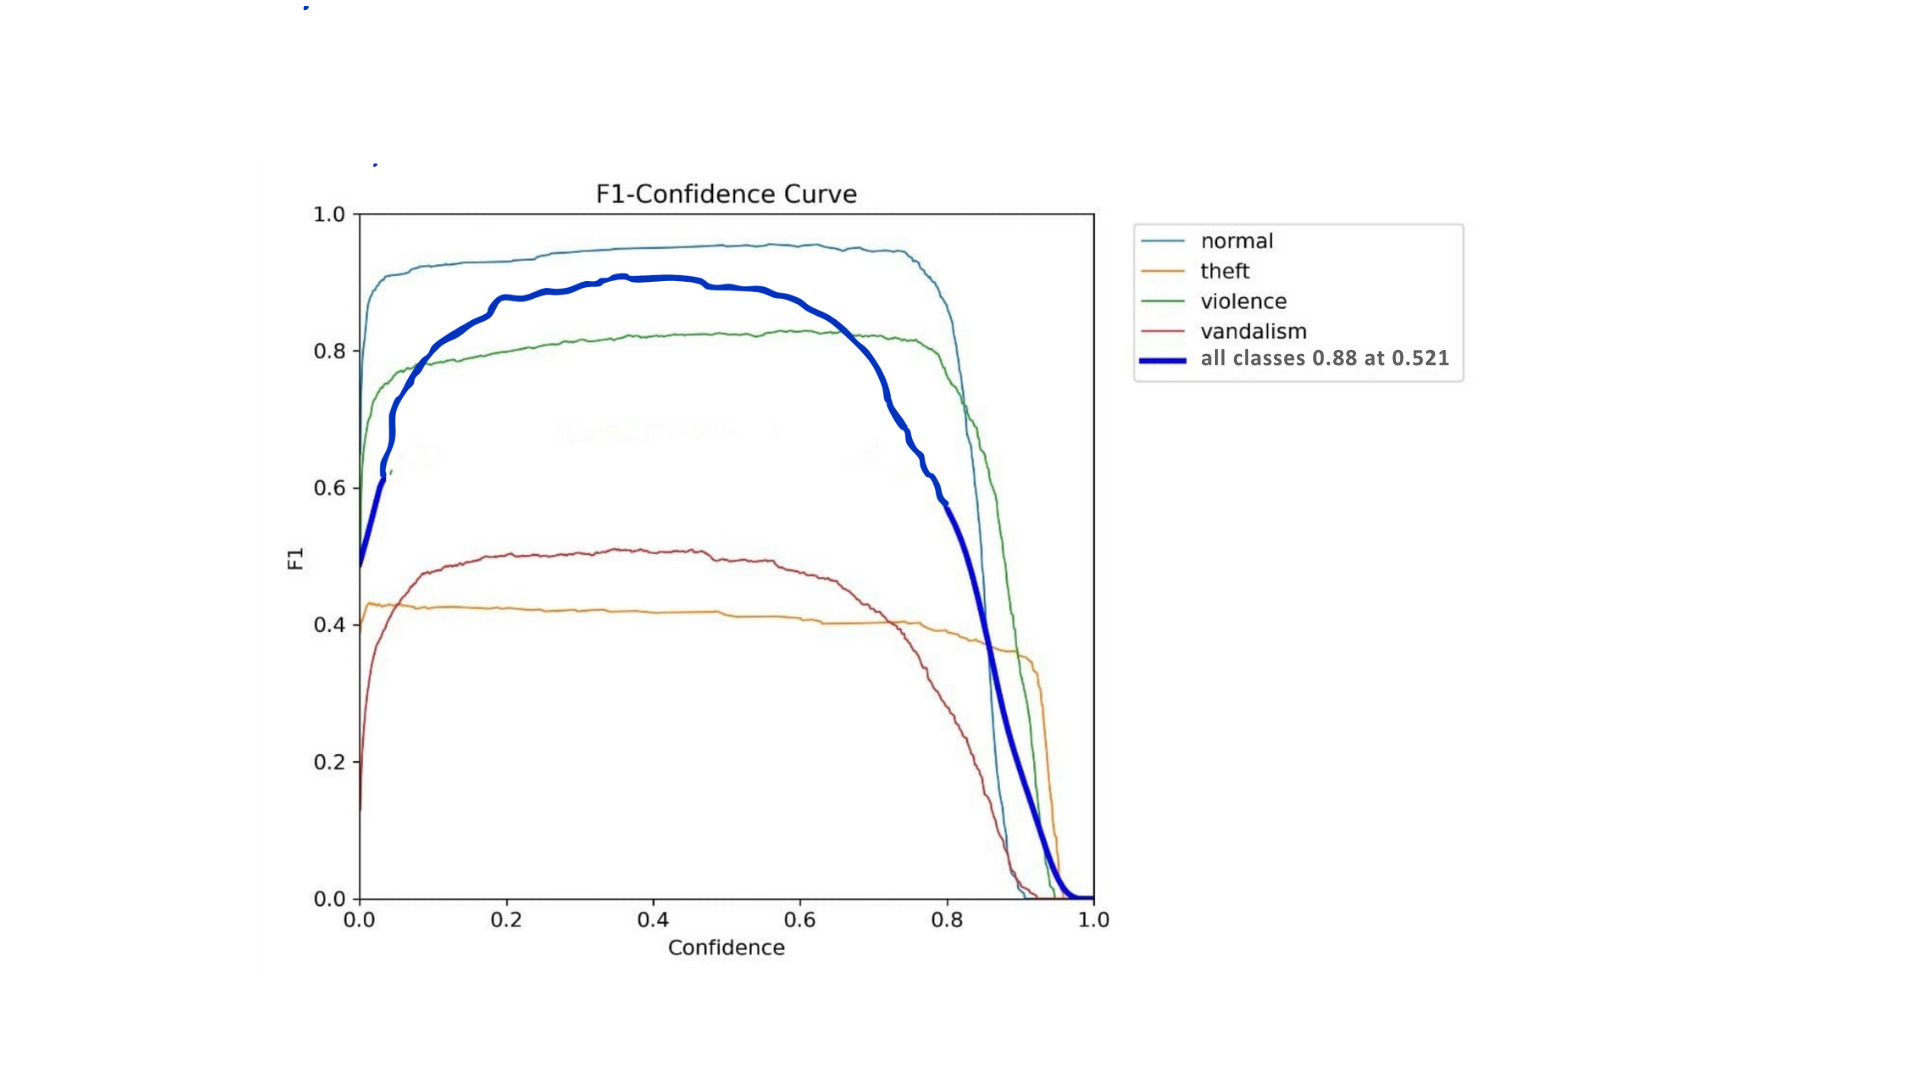
\includegraphics[width=0.85\textwidth]{f1_curve.png}
\caption{F1-confidence curve for the YOLOv11 model across all behavior classes.}
\label{fig:f1}
\end{figure}

\subsection{Confusion Matrix}

Figures~\ref{fig:cm} and~\ref{fig:cmn} present the raw and normalized confusion matrices for the detection model, respectively. The diagonal dominance confirms strong per-class discrimination. Minor confusion is observed between adjacent activity classes (e.g., fighting and vandalism), which share overlapping spatial features.

\begin{figure}[t]
\centering
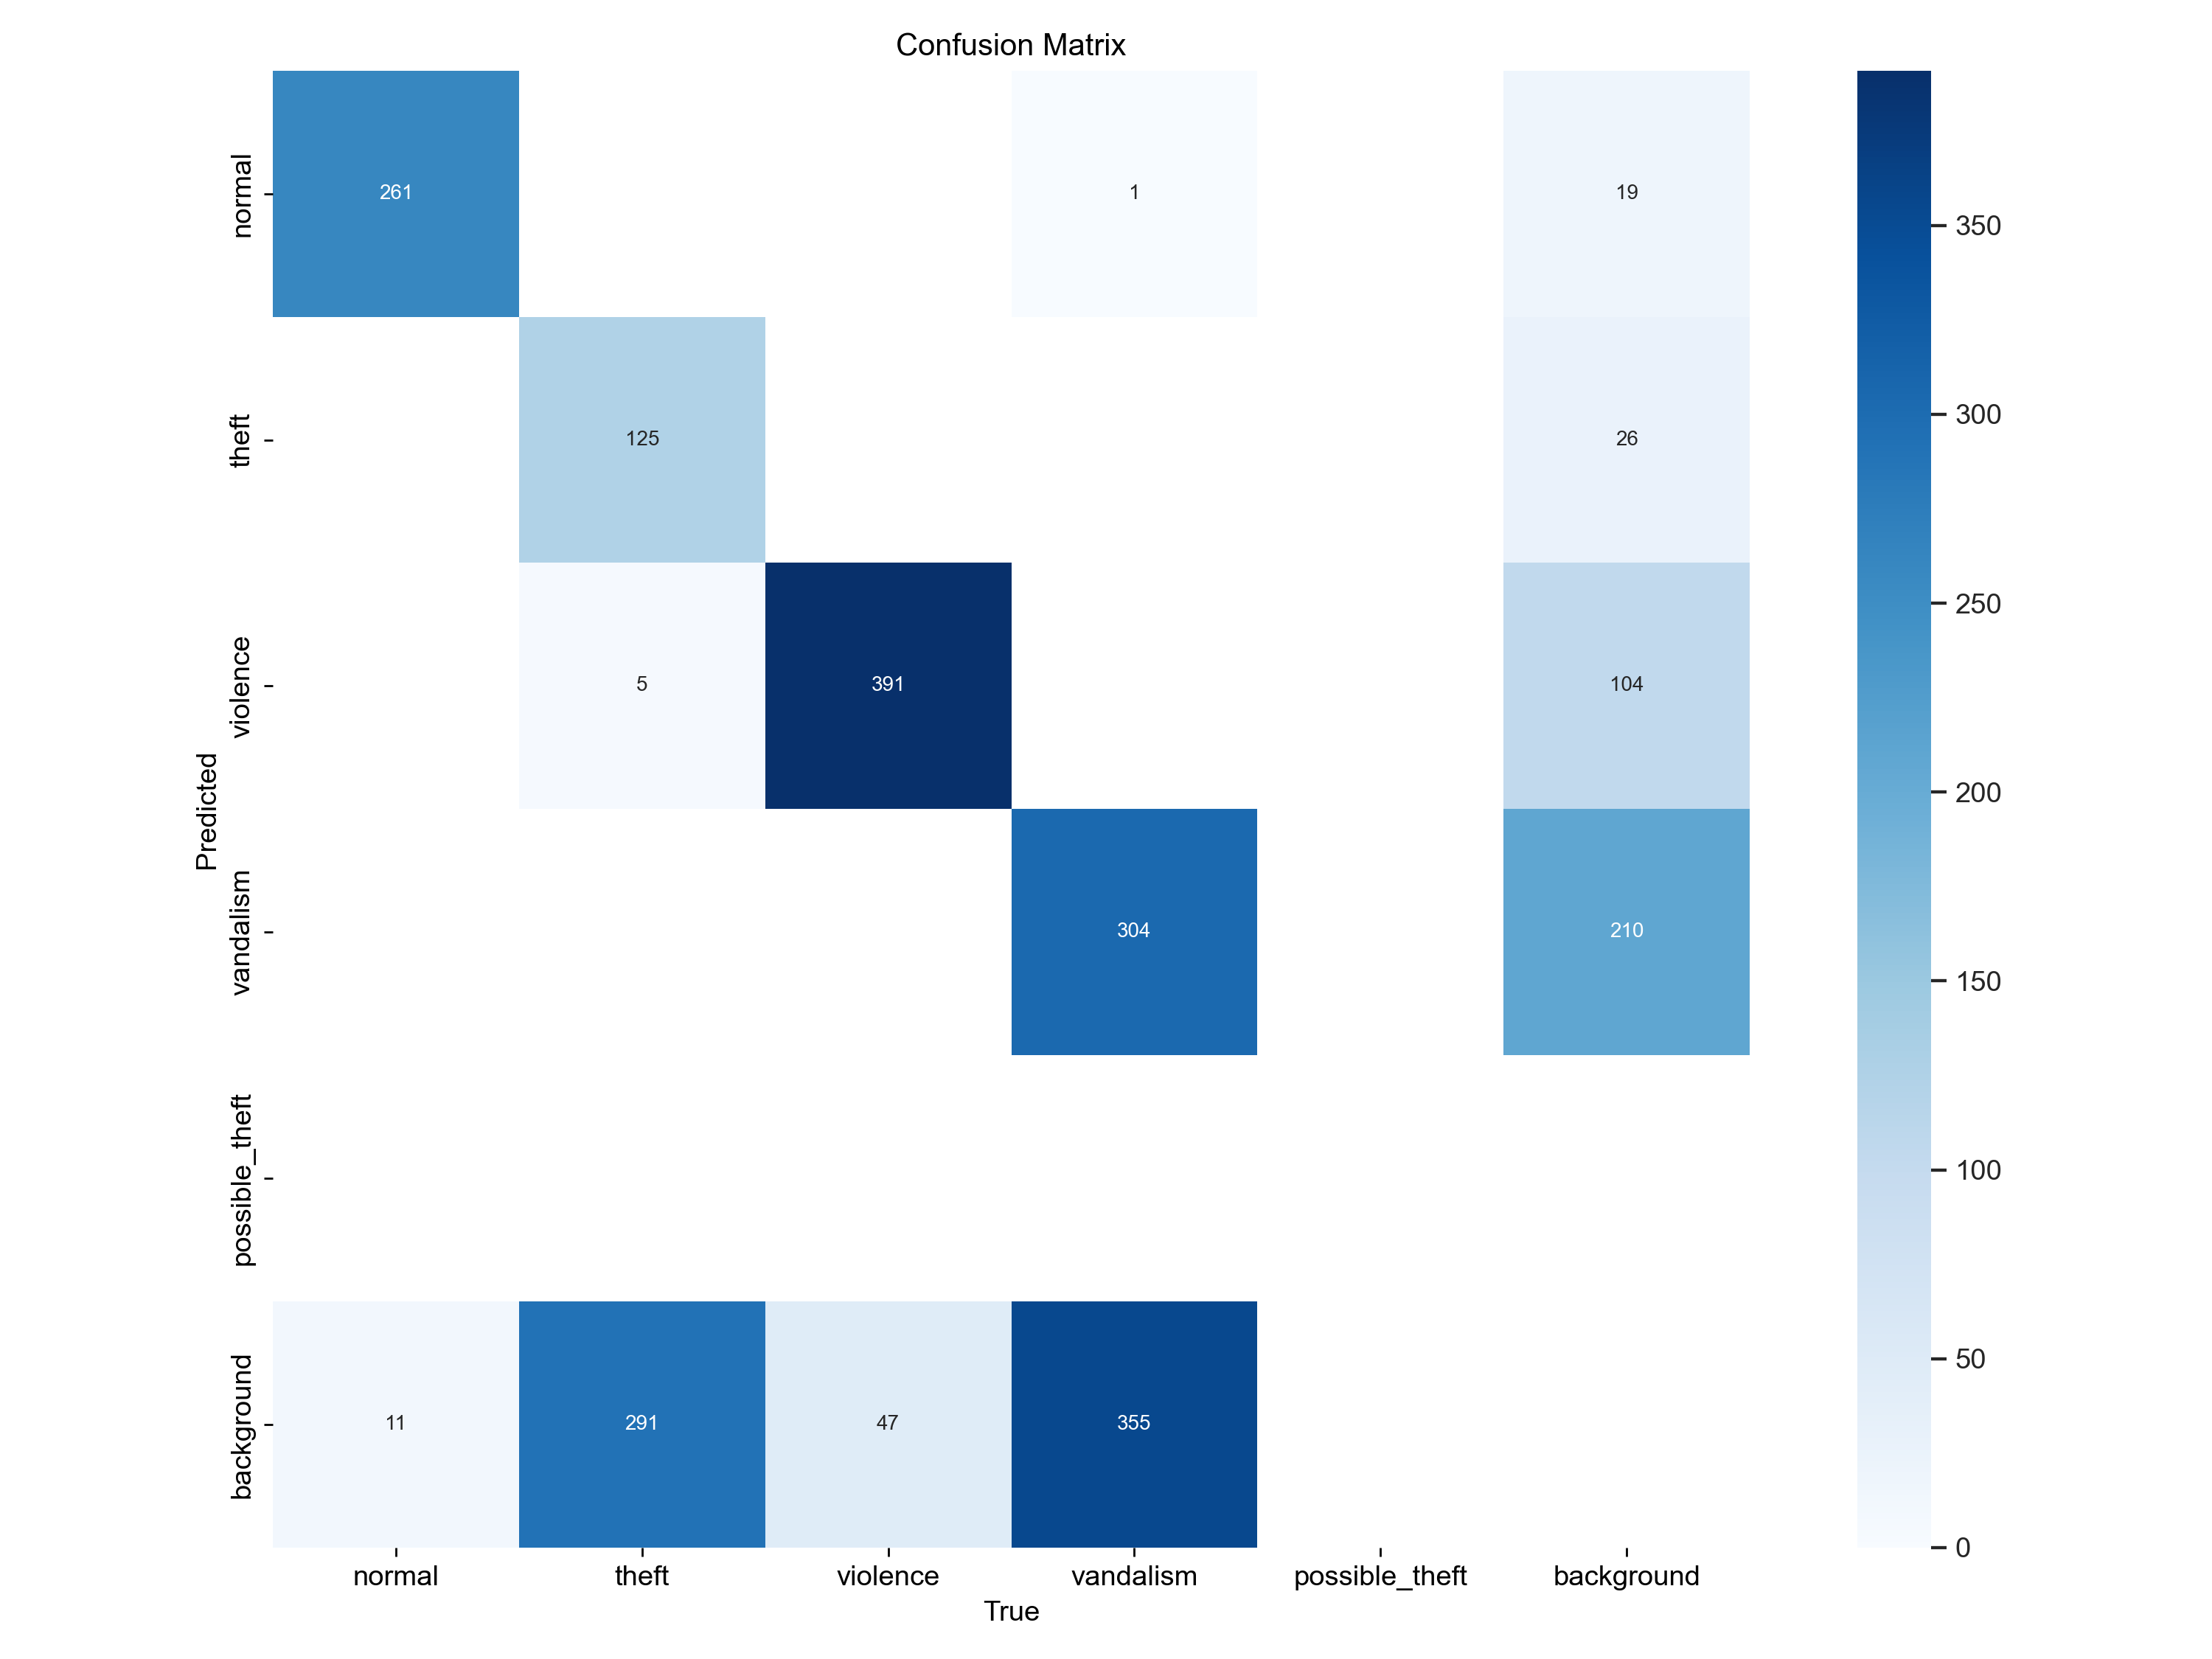
\includegraphics[width=0.75\textwidth]{confusion_matrix.png}
\caption{Confusion matrix (raw counts) of the YOLOv11 model.}
\label{fig:cm}
\end{figure}

\begin{figure}[t]
\centering
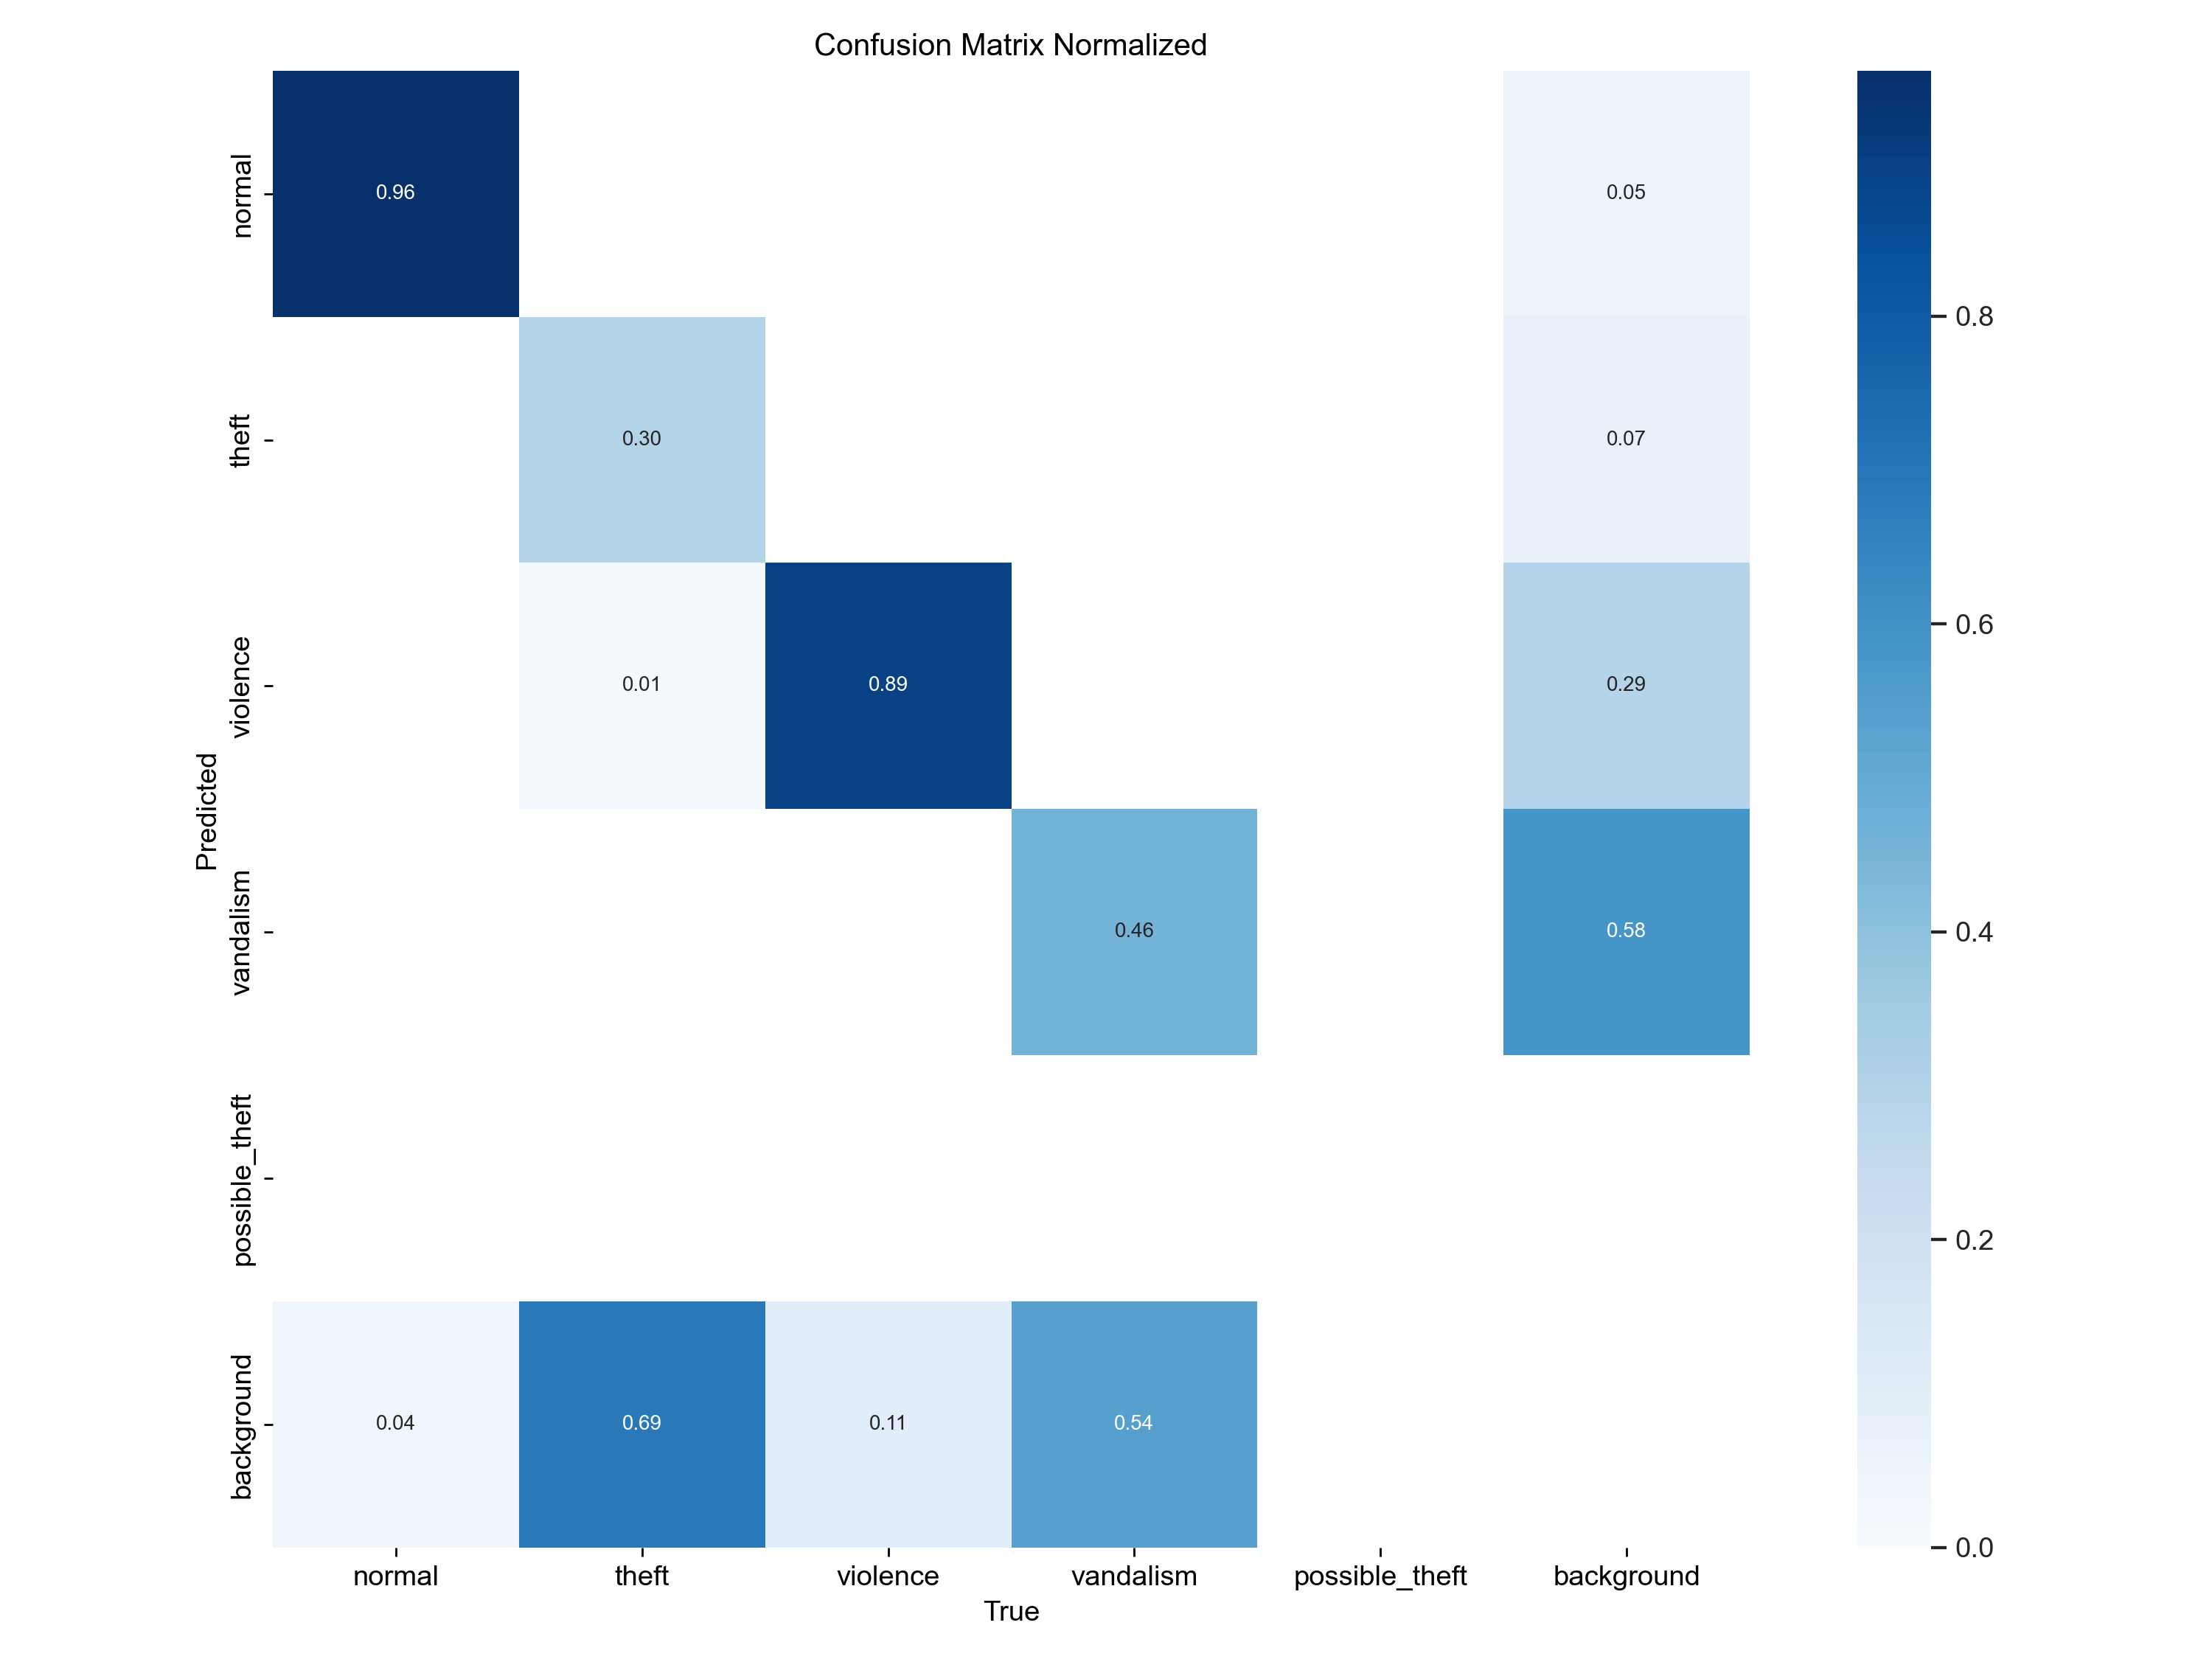
\includegraphics[width=0.75\textwidth]{confusion_matrix_normalized.png}
\caption{Normalized confusion matrix of the YOLOv11 model.}
\label{fig:cmn}
\end{figure}

\subsection{CNN+LSTM Video Classification Performance}

The InceptionV3+GRU video classifier achieves a test classification accuracy of approximately 88\% on held-out video clips and 82\% per-frame compliance accuracy, demonstrating effective temporal modeling of behavior patterns across sequences.

\subsection{Inference Speed}

On the NVIDIA GeForce GTX 1650, the YOLOv11 detector achieves an average inference time of approximately 25--28~ms per frame at $640 \times 640$ resolution, corresponding to roughly 35--40 FPS before preprocessing overhead. This confirms real-time applicability on consumer-grade hardware.

\section{Conclusion}
\label{sec:conclusion}

This paper presented a hybrid real-time human behavior analysis system combining YOLOv11 frame-level detection and an InceptionV3+GRU video classifier for identifying theft, vandalism, fighting, and normal behavior in surveillance footage. The YOLOv11 component achieves mAP@50 of 0.96 with precision 0.95 and recall 0.93. The video classifier achieves 88\% accuracy on held-out clips. Integrated Telegram-based alerting enables automated real-time incident response.

Future work will focus on: (1) expanding the dataset with more diverse scenarios and viewpoints, (2) incorporating optical flow as an additional input modality, (3) exploring lightweight transformer architectures for improved temporal modeling, and (4) deploying the system on edge devices such as NVIDIA Jetson for embedded surveillance applications.

\section*{Disclosure of Interests}

The authors declare no competing interests.

\begin{thebibliography}{8}

\bibitem{redmon2016}
Redmon, J., Divvala, S., Girshick, R., Farhadi, A.: You Only Look Once: Unified, Real-Time Object Detection. In: CVPR, pp. 779--788 (2016)

\bibitem{jocher2023}
Jocher, G., Chaurasia, A., Qiu, J.: Ultralytics YOLO. \url{https://github.com/ultralytics/ultralytics} (2023)

\bibitem{khanam2024}
Khanam, R., Hussain, M.: YOLOv11: An Overview of the Key Architectural Enhancements. arXiv:2410.17725 (2024)

\bibitem{he2016}
He, K., Zhang, X., Ren, S., Sun, J.: Deep Residual Learning for Image Recognition. In: CVPR, pp. 770--778 (2016)

\bibitem{simonyan2015}
Simonyan, K., Zisserman, A.: Very Deep Convolutional Networks for Large-Scale Image Recognition. In: ICLR (2015)

\bibitem{donahue2015}
Donahue, J., et al.: Long-Term Recurrent Convolutional Networks for Visual Recognition and Description. In: CVPR, pp. 2625--2634 (2015)

\bibitem{szegedy2016}
Szegedy, C., Vanhoucke, V., Ioffe, S., Shlens, J., Wojna, Z.: Rethinking the Inception Architecture for Computer Vision. In: CVPR, pp. 2818--2826 (2016)

\bibitem{chung2014}
Chung, J., Gulcehre, C., Cho, K., Bengio, Y.: Empirical Evaluation of Gated Recurrent Neural Networks on Sequence Modeling. arXiv:1412.3555 (2014)

\end{thebibliography}

\end{document}
